\documentclass{tufte-handout}

%\date{28 March 2010} % without \date command, current date is supplied

%\geometry{showframe} % display margins for debugging page layout

\usepackage{graphicx} % allow embedded images
  \setkeys{Gin}{width=\linewidth,totalheight=\textheight,keepaspectratio}
  \graphicspath{{graphics/}} % set of paths to search for images
\usepackage{amsmath}  % extended mathematics
\usepackage{booktabs} % book-quality tables
\usepackage{units}    % non-stacked fractions and better unit spacing
\usepackage{multicol} % multiple column layout facilities
\usepackage{lipsum}   % filler text
\usepackage{fancyvrb} % extended verbatim environments
  \fvset{fontsize=\normalsize}% default font size for fancy-verbatim environments

% Standardize command font styles and environments
\newcommand{\doccmd}[1]{\texttt{\textbackslash#1}}% command name -- adds backslash automatically
\newcommand{\docopt}[1]{\ensuremath{\langle}\textrm{\textit{#1}}\ensuremath{\rangle}}% optional command argument
\newcommand{\docarg}[1]{\textrm{\textit{#1}}}% (required) command argument
\newcommand{\docenv}[1]{\textsf{#1}}% environment name
\newcommand{\docpkg}[1]{\texttt{#1}}% package name
\newcommand{\doccls}[1]{\texttt{#1}}% document class name
\newcommand{\docclsopt}[1]{\texttt{#1}}% document class option name
\newenvironment{docspec}{\begin{quote}\noindent}{\end{quote}}% command specification environment

\geometry{textwidth=.6\paperwidth}
\geometry{bottom=1.5cm}
\geometry{top=1.5cm}

\usepackage[utf8]{inputenc}
\usepackage{amssymb}

\newcommand{\Hau}{\text{Hau}}
\newcommand{\End}{\text{End}}
\newcommand{\inlinedef}[1]{\textcolor{purple}{#1}}
\newcommand{\id}{\text{id}}
\newcommand{\cf}{$\rightarrow$~}
\newcommand{\mat}[1]{\mathbf{#1}}


\usepackage{xcolor}

% \newenvironment{definition}[1]{
%  \colorbox{blue!30}{blue} \paragraph{#1}
% }{
%   .
% }


\newenvironment{definition}[2]{%
\par
\noindent
\paragraph{\colorbox{purple!30}{Def. #1}} (\textit{#2}) \\
\vspace{0.5em}
\noindent
}
{}


\newenvironment{exercise}[2]{%
  \par
  \noindent
  \paragraph{\colorbox{orange!30}{Ex. #1} ~ \textcolor{gray}{#2}} 
  \vspace{0.5em}
  \noindent
}{}

\newenvironment{theorem}[2]{%
  \par
  \noindent
  \paragraph{\colorbox{orange!30}{Th. #1}} (\textit{#2})\\
  \vspace{0.5em}
  \noindent
}{}

\newenvironment{algorithm}[2]{%
  \par
  \noindent
  \paragraph{\colorbox{blue!30}{Alg. #1}} (\textit{#2}) \\
  \vspace{0.5em}
  \noindent
}{}

\newenvironment{proof}{%
  \par
  \noindent
  \hfill\begin{minipage}{\dimexpr\textwidth-1em}
  \vspace{1em}
  \paragraph{Proof: }
  \noindent
}{
  \xdef\tpd{\the\prevdepth}
  \vspace{1em}
  \end{minipage}
}

\usepackage{enumitem}

\newcommand{\nn}{\ensuremath{\mathbb{N}}}

\newcommand{\len}{\ensuremath{\text{len}}}
\newcommand{\enc}{\ensuremath{\text{enc}}}
\newcommand{\leqae}{\ensuremath{\leq_{ae}}}

\newcommand{\twotdspace}{\textsc{2-t-dspace}}
\newcommand{\onetdspace}{\textsc{1-t-dspace}}

\newcommand{\bigO}{\ensuremath{\mathcal{O}}}


\makeatletter
\renewcommand{\paragraph}{%
  \@startsection{paragraph}{4}%
  {\z@}{0.00ex \@plus 1ex \@minus .2ex}{-1em}%
  {\normalfont\normalsize\bfseries}%
}
\makeatother

\begin{document}

\textsc{Stress Minimization} --- User Manual

  \setlength{\parindent}{0em}
  \setlength{\parskip}{0.75em}

  \section{Introduction}
  \subsection{Overview}
  This layout provides a graph layouting algorithm to \textsc{Vanted}. The
  algorithm is based on the concept of minimising an objective value of the
  network, its so-called \textit{stress}
  \sidenote{Gansner, Koren, North: \textit{Graph Drawing by Stress
      Majorization}}
  \sidenote{Mader: \textit{Drawing Dynamic Graphs by Stress Minimization}}.
  It tries to assign positions to nodes
  such that the distances in the drawing between two node matches their
  graph-theoretical distance \sidenote{i.e. the number of edges one has to walk
    to get from node to the other}.

  For the stress measure, one can derive a (convex) quadratic form $T$ that majorizes
  it. Optimising $T$ yields an improved layout. The algorithm iteratively
  optimises majorants until the stress reduction falls below a given threshold.
  \begin{marginfigure}
    \centering
    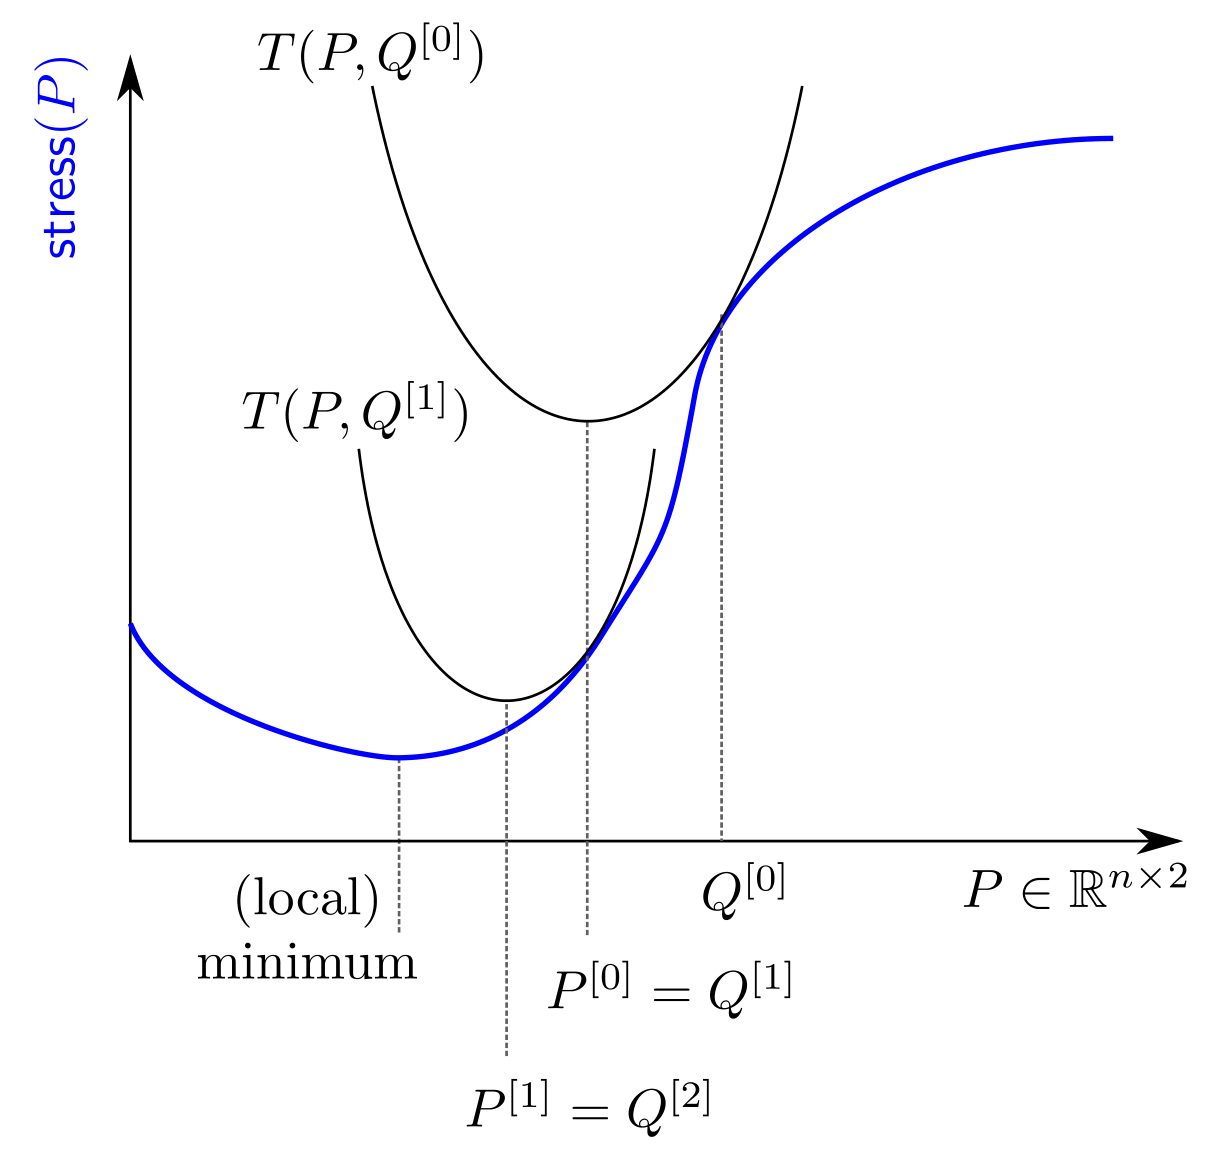
\includegraphics[width=0.9\textwidth]{iterative-optimisation}
    \caption{Iterative optimisation by finding majorants of increasing quality.}
  \end{marginfigure} 

  The algorithm implements the formulation of Mader et al.
  
  The algorithm can configured to compute a full optimisation or an
  approximation using a landmark strategy.

  \subsection{Dependencies}

  \begin{itemize}
  \item Apache Commons Math 3.0 API (packaged with the Add-On).
  \item The plugin requires \textsc{Vanted} 2.6.5, including the libraries it is
    based upon.
  \end{itemize}
  \subsection{License}
    This software is licensed under \textit{GNU General
      Public License, version 3}
    \sidenote[][1em]{\url{https://github.com/xnhp/vanted-addon-sm/blob/master/LICENSE.txt}}.


    \section{Working with the Stress Minimization Add-On}

   \paragraph{Auto Redraw} If checked, after each iteration of the optimiser,
   the view will be updated with the current layout. Note that this may
   introduce significant lag. This option can be toggled on and off during the
   execution of the algorithm.

   \paragraph{Preprocessing} Whether the currently displayed layout or a random
   layout should be used as an inital layout for the iterative optimisation.

   \paragraph{Method} Whether to consider the full set of nodes for calculating
   and optimising the stress measure or to follow a landmark strategy. In the
   latter case, landmarks are selected using the \textsc{MaxMin} strategy.
   \sidenote{The next landmark is the one with the maximum shortest distance to
     any other previously selected landmark. The first landmark is the node with
   the highest degree.}
   After an optimised layout for the landmarks has been found, other nodes are
   placed around the landmarks in barycentric fashion.

 \paragraph{Weight exponent} Dissimilarities between the current layout and the
 shortest-path distance can be weighted by $d_{ij}^{-\alpha}$ where $d_{ij}$ is
 the shortest-path distance between nodes $i$ and $j$. $\alpha=0$, also called
 \textit{absolute stress}, results in a layout that emphasises larger distances.
 Local structures might not be clearly distinguised. $\alpha \in \{-1, -2\}$,
 also called \textit{semi-proportional} and \textit{proportional} stress, resp.,
 will not represent large dissimilarities faithfully but down-weight them.
 However, local structures will be more clearly revealed.

 \paragraph{Stress change threshold} If the total stress change in an iteration
 falls below this amount, the computation terminates.

 \paragraph{Node movement threshold} If the maximum movement of a node falls
 below this value, the computation terminates.

 \paragraph{Maximum number of iterations} The maximum number of optimisation
 cycles to perform.
    

\end{document}
